\documentclass[12pt,a4paper]{article}

\usepackage{tikz}
\usepackage[margin=2cm]{geometry}
\usetikzlibrary{shapes, arrows}
\usetikzlibrary{mindmap}


\begin{document}

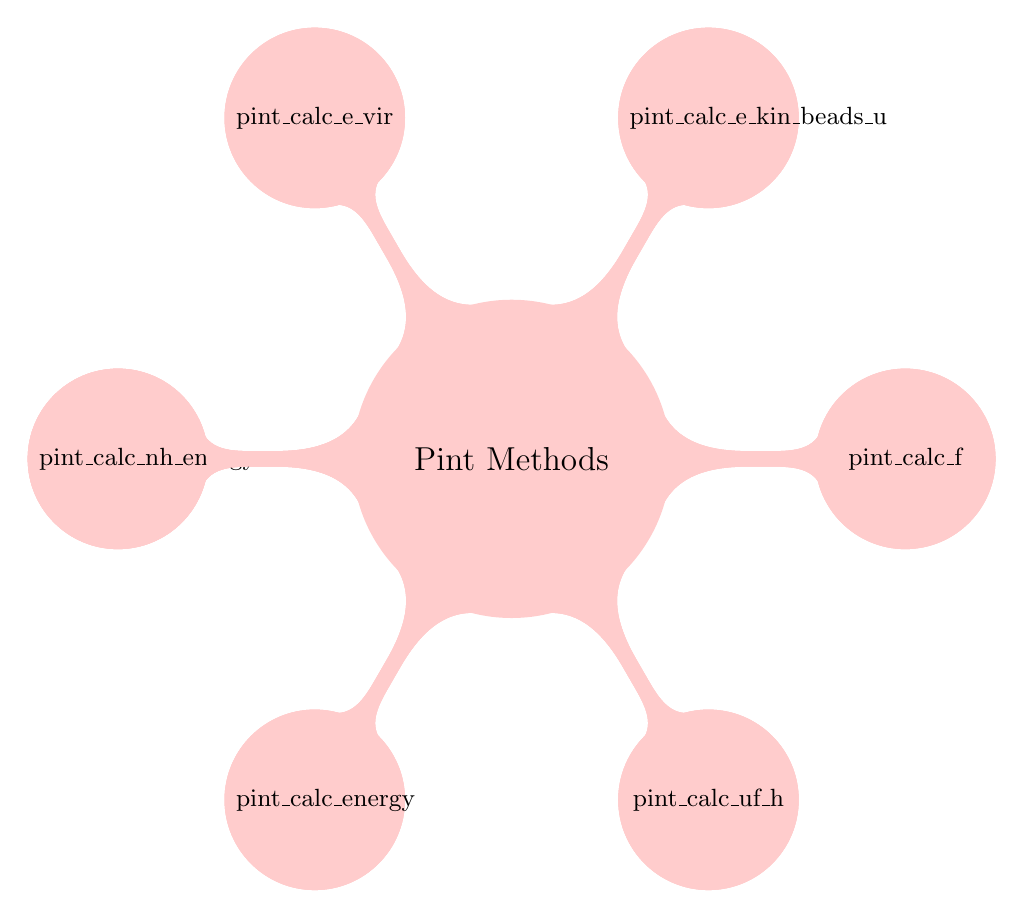
\begin{tikzpicture}[mindmap, every node/.style=concept, concept color=red!20, grow cyclic]
\node [root concept]{Pint Methods}
child { node { pint\_create }}
child { node { pint\_retain }}
child { node { pint\_release }}
child { node { pint\_test }}
child { node { do\_pint\_run }}
child { node { pint\_init }}
child { node { pint\_init\_x }}
child { node { pint\_init\_v }}
child { node { pint\_init\_t }}
child { node { pint\_init\_f }}
child { node { pint\_do\_run }}
child { node { pint\_run\_scan }}
child { node { pint\_step }}
child { node { pint\_calc\_energy }}
child { node { pint\_calc\_uf\_h }}
child { node { pint\_calc\_f }}
child { node { pint\_calc\_e\_kin\_beads\_u }}
child { node { pint\_calc\_e\_vir }}
child { node { pint\_calc\_nh\_energy }};
\end{tikzpicture}

\end{document}